\documentclass{standalone}
\usepackage{tikz}

\begin{document}
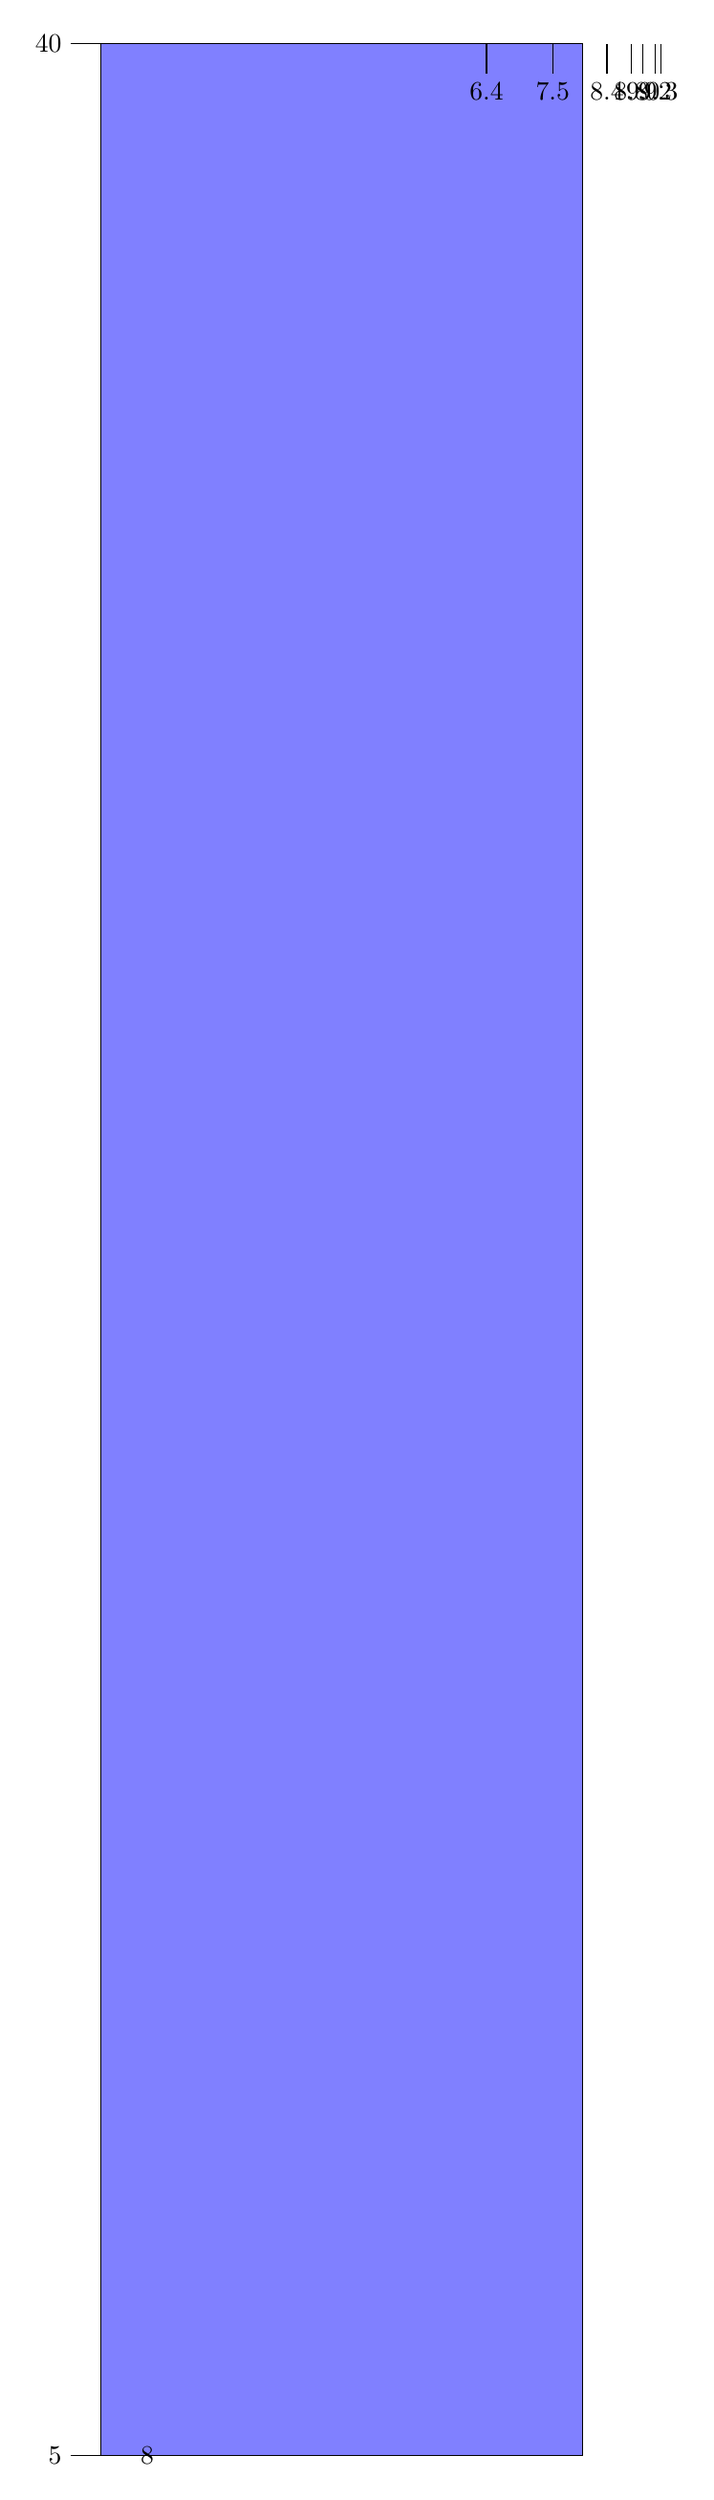
\begin{tikzpicture}[scale=0.8]
    % Draw the rectangle
    \draw[fill=blue!50] (0,0) -- (8,0) -- (8,40) -- (0,40) -- cycle;
    
    % Draw the top horizontal line with labels
    \draw (0,40) -- (8,40);
    \foreach \x/\l in {6.4/6.4, 7.5/7.5, 8.4/8.4, 9.0/9.0, 9.3/9.3, 9.2/9.2, 8.8/8.8} {
        \draw (\x,40) -- ++(0,-0.5) node[below] {\l};
    }
    
    % Draw the vertical lines with labels
    \foreach \y/\l in {0/5, 40/40} {
        \draw (0,\y) -- ++(-0.5,0) node[left] {\l};
    }
    
    % Draw the bottom horizontal line with labels
    \draw (0,0) -- (8,0);
    \foreach \x/\l in {0/8} {
        \draw (\x,0) -- ++(0.5,0) node[right] {\l};
    }
\end{tikzpicture}
\end{document}